\documentclass{book}

\usepackage{amsmath} %maths
\usepackage{enumerate} %change of the label of enumerate
\usepackage{booktabs} %toprule series
\usepackage{graphicx} %figure

\begin{document}

\title{THE SAMPLE OF LATEX}
\author{ENGLISH EDITION}
\date{}
\maketitle

\tableofcontents

\mainmatter

\part{Words  Symbols and Mathematics}

\chapter{Words}

this is my book.this is my book.this is my book.this is my book.this is my book.this is my book.this is my book.this is my book.this is my book.this is my book.this is my book.this is my book.this is my book.this is my book.this is my book.this is my book.this is my book.this is my book.this is my book.this is my book.this is my book.


\chapter{Symbols and Mathematics:Far to go}

\[a^2+b^2=c^2\]

$$a^2+b^2=c^2$$

\$,\%,\^X,$\backslash$,\& ,$\setminus$,$\backslash$

this is my book.$a^2+b^2=c^2$this is my book.

$$\sum^\infty_{i=1} \lbrace (x^2+y^2) \rbrace $$
$$\overbrace{abcd}$$
$$\frac{a^2}{b^2}$$
$$\mathop{abcd}^1_2$$
$${abcd}^1_2$$

\begin{equation}
a^2+b^2=c^2\\
%d^2+e^2=f^2 %?
\end{equation}


\part{Tables and Figures}

\chapter{Tables}

\section{Enumerations}

\begin{itemize}
\item first 
\begin{itemize}
\item first 1
\item first 2
\end{itemize}
\item second
\item third
\end{itemize}

\begin{enumerate}
\item first 
\begin{enumerate}
\item first 1
\item first 2
\end{enumerate}
\item second
\item third
\end{enumerate}

\begin{enumerate}[\bfseries A] %bold font series of characters 
\item first 
\begin{enumerate}[\sffamily a.] %\usepackage{enumerate}
\item first 1
\item first 2
\end{enumerate}
\item second
\item third
\end{enumerate}

\section{Tables}

\begin{flushright}
\begin{tabular}{|c|l|r|}
3242&3241&32\\
321&421412&32\\
\end{tabular}
\end{flushright}

\begin{center}
\begin{tabular}{clr}
\hline 
\vline
3242&3241&32\\
\hline
321&421412&32\\
\cline{2-3}
3232&8686&423\\
\hline 
\end{tabular}
\end{center}

\begin{table}[h]
\centering
\begin{tabular}{ccc}
\toprule		%\usepackage{booktabs}
3242&3241&32\\
\midrule
321&421412&32\\
3232&8686&423\\
\bottomrule
\end{tabular}
\caption{this is a standard table}
\end{table}

\chapter{Figures} %\usepackage{graphicx}

\begin{figure}[h]
\centering
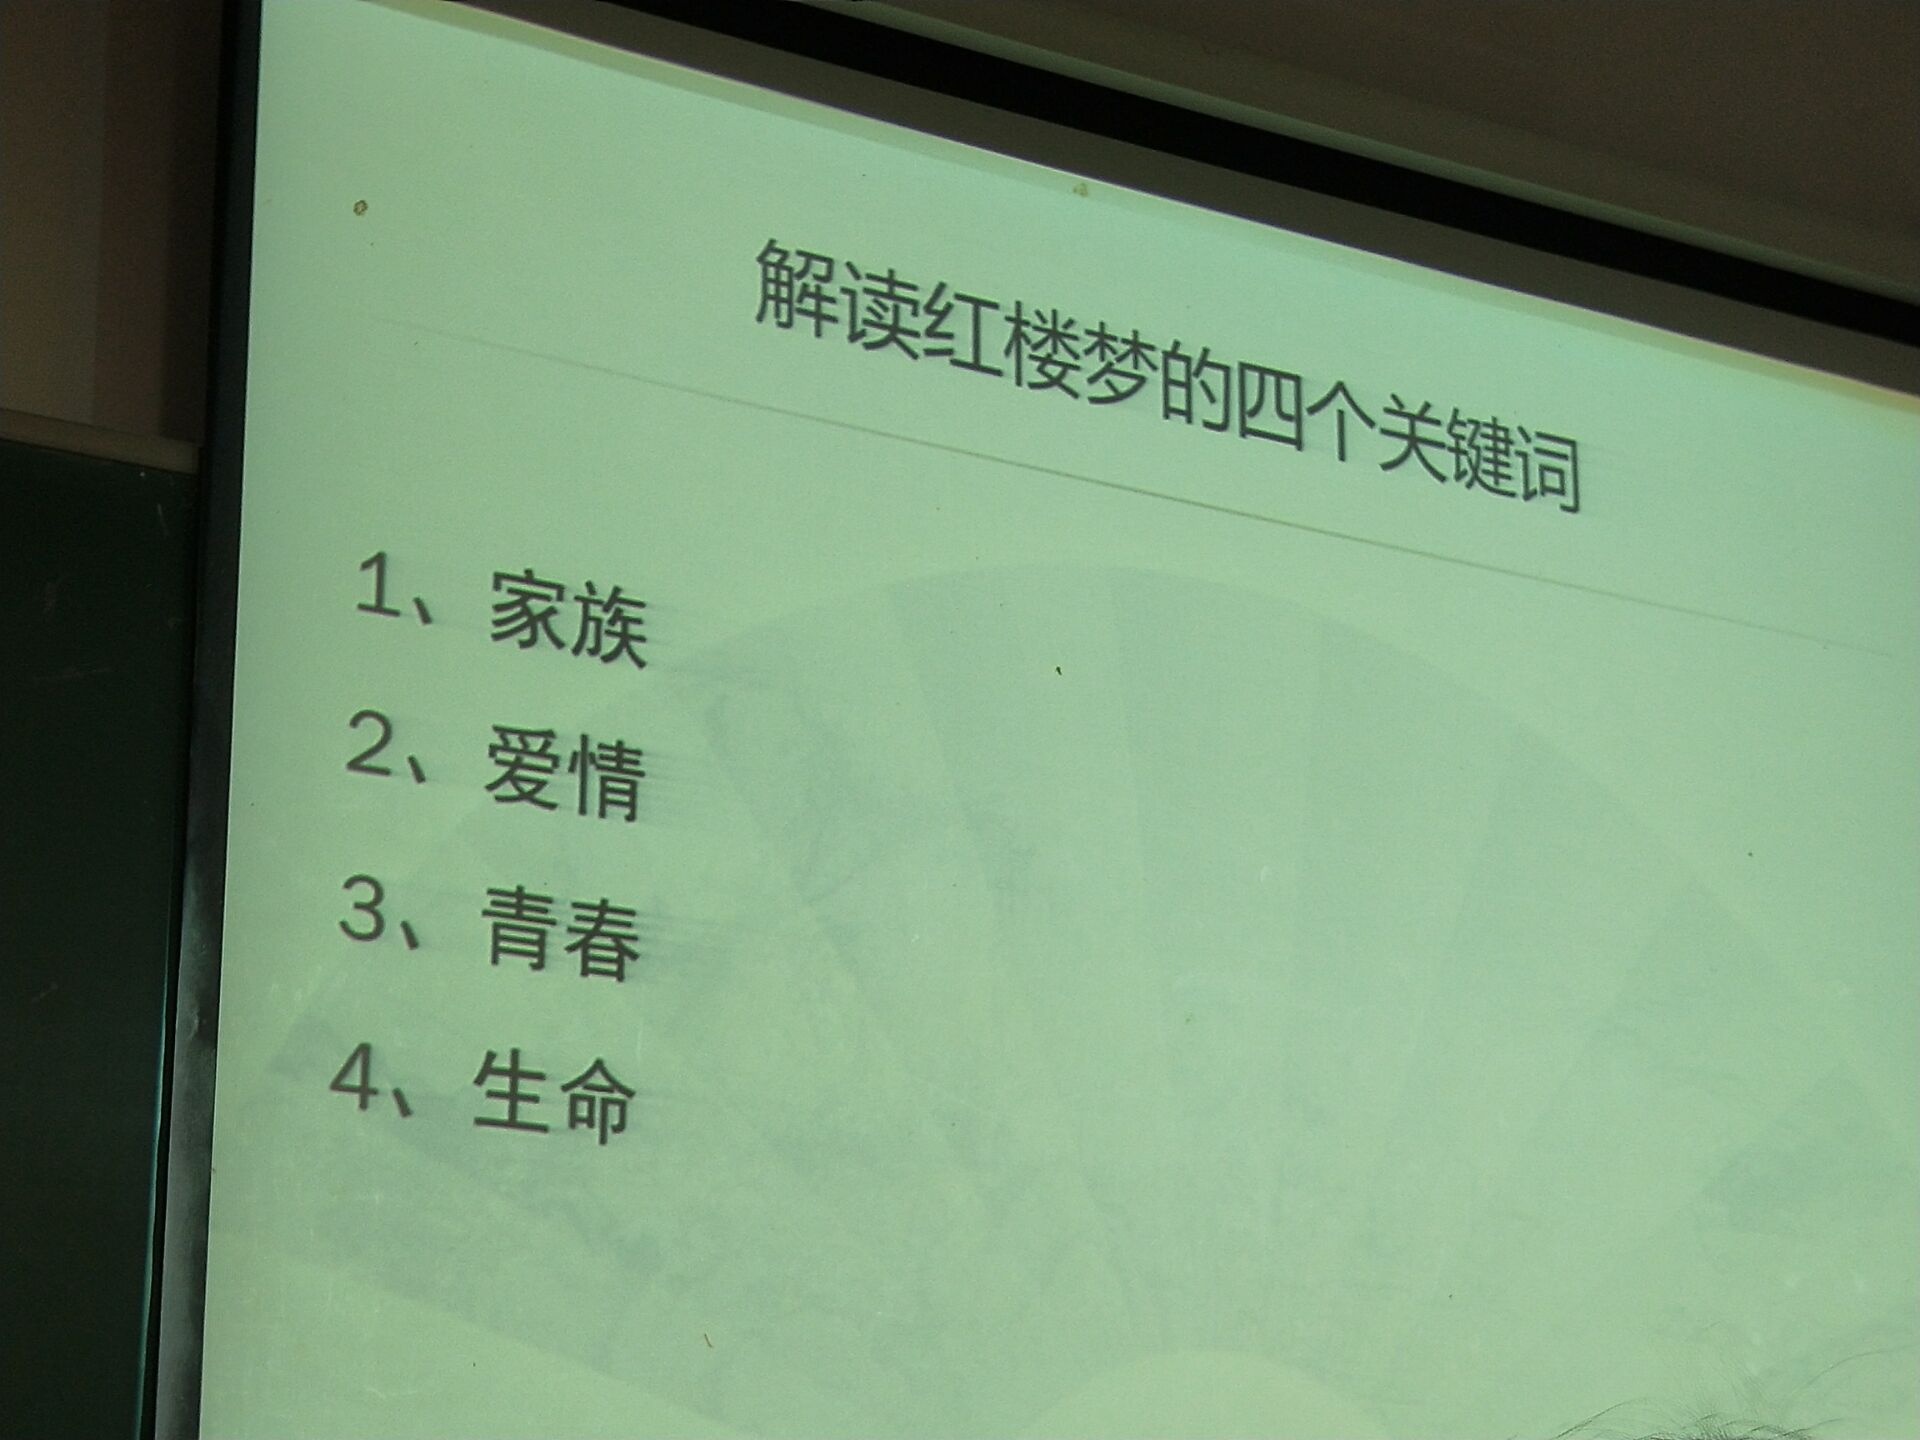
\includegraphics[scale=0.1]{English_edition.jpg}
\caption{this is an important figure}
\end{figure}

\newpage
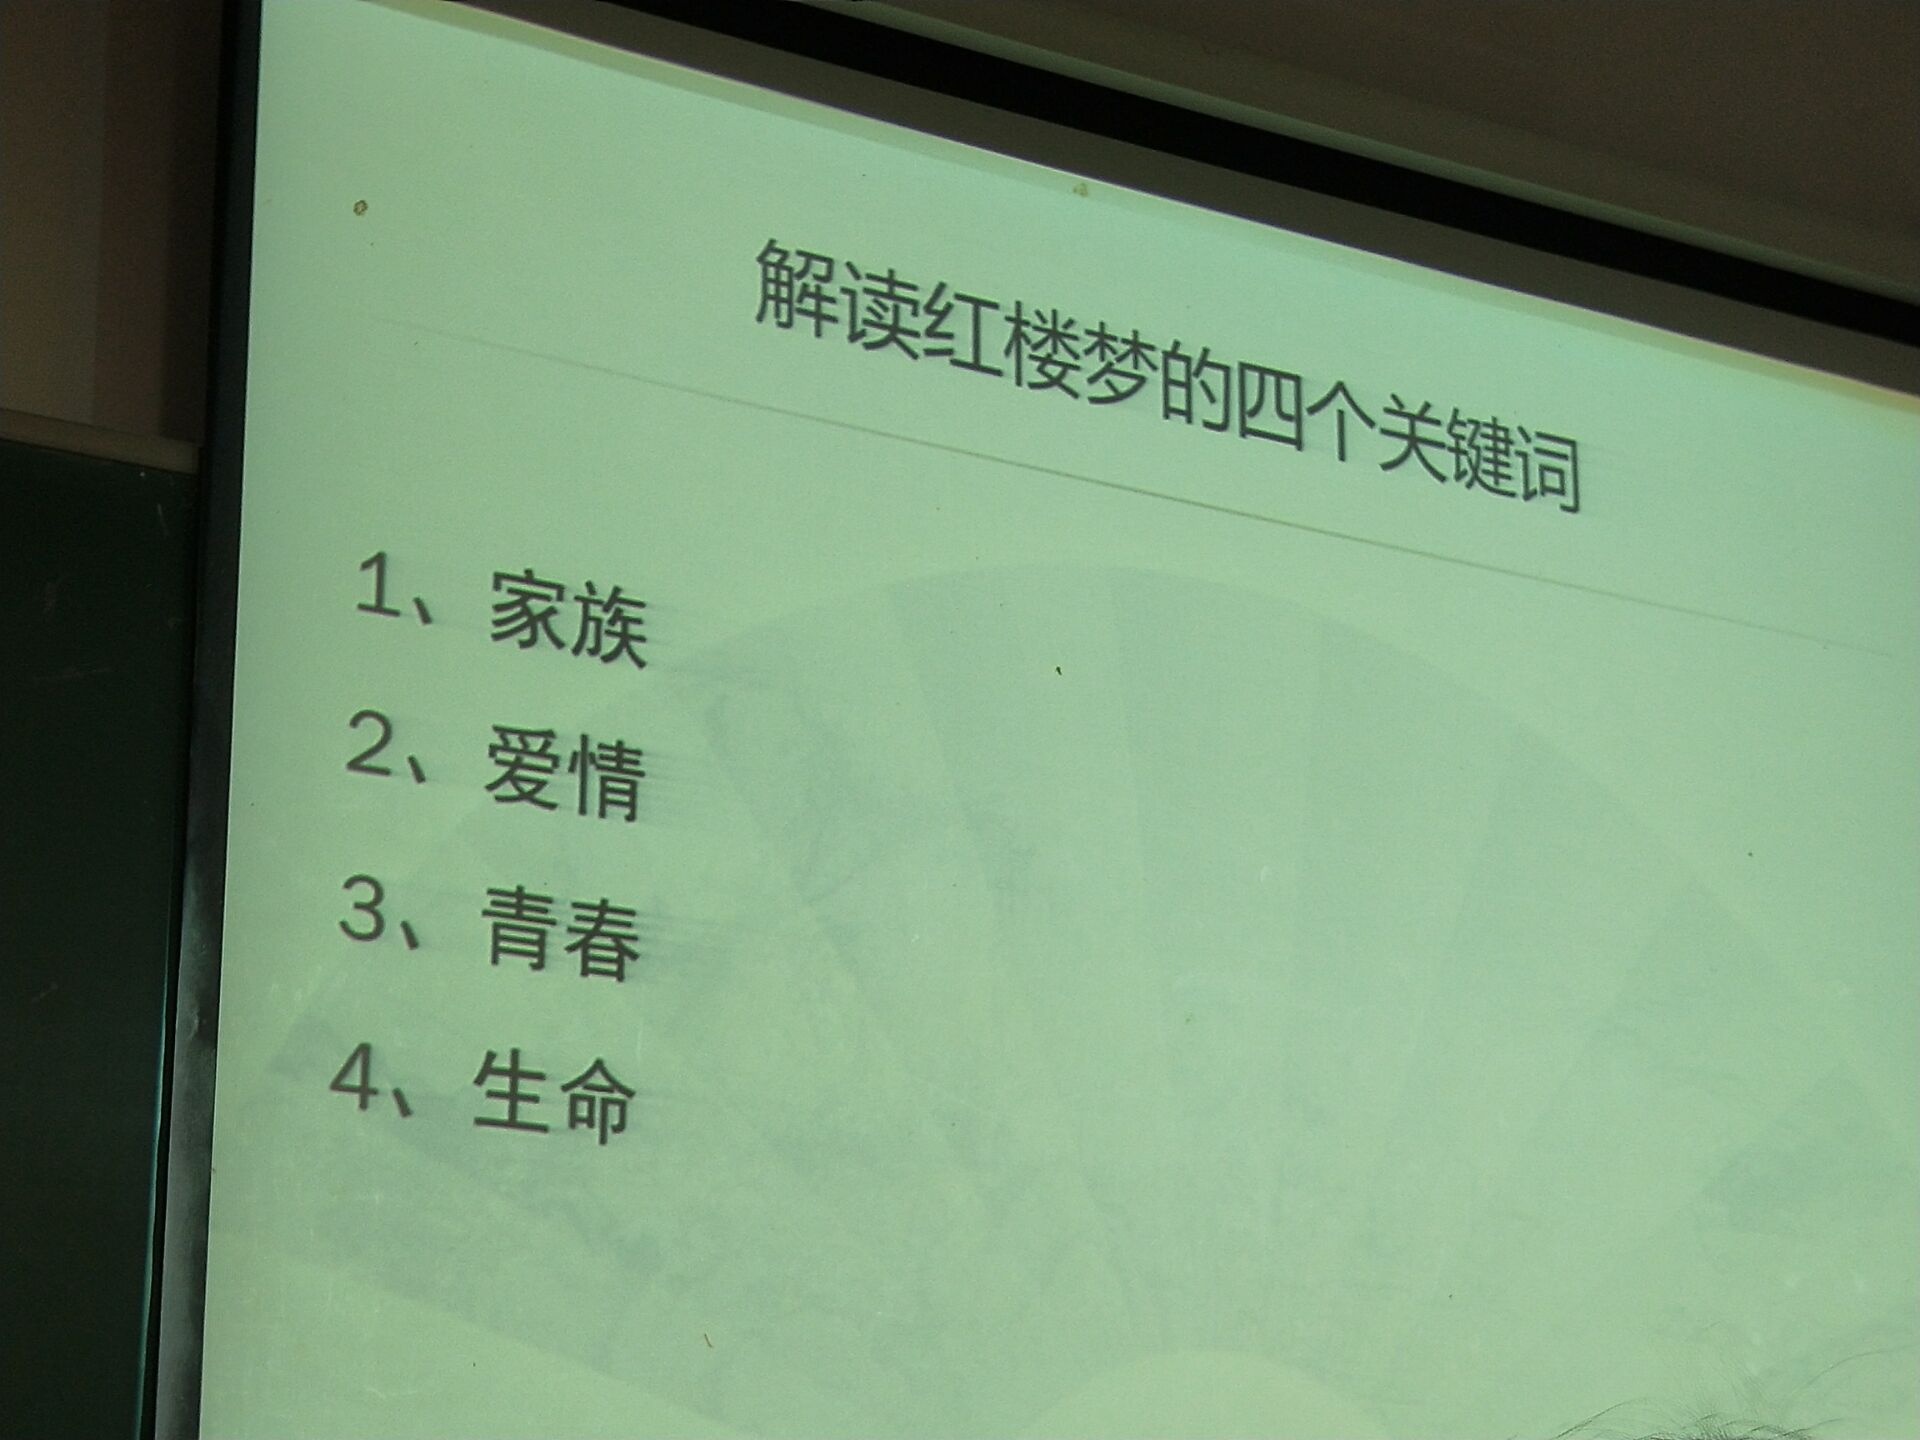
\includegraphics[scale=0.1]{English_edition.jpg} 

\begin{figure}[h]
\centering
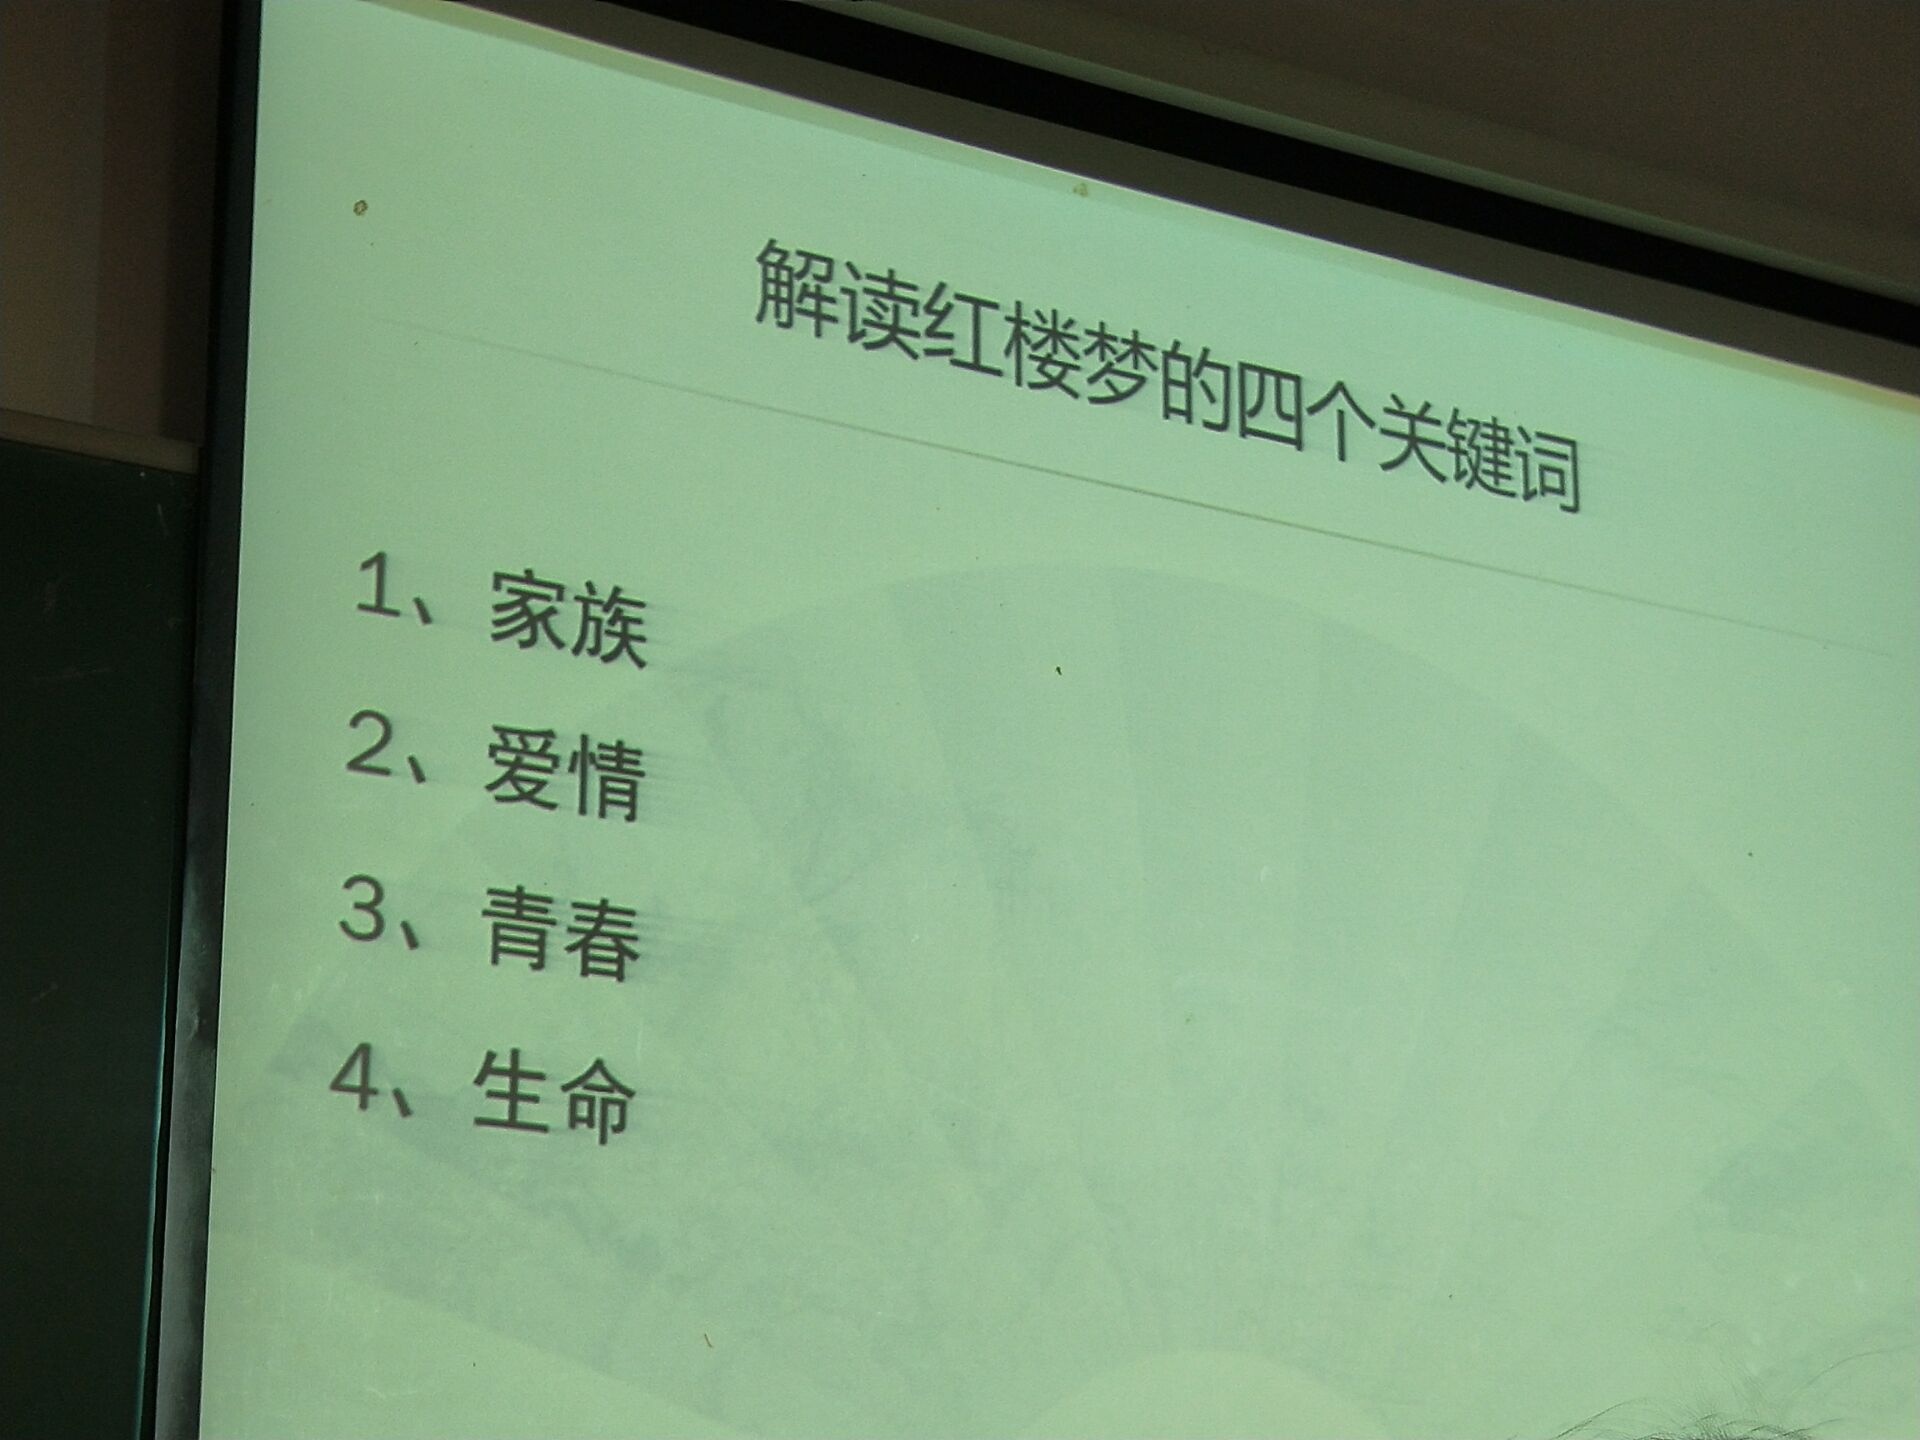
\includegraphics[scale=0.1]{English_edition.jpg}
\caption{this is an important figure}
\end{figure}
\end{document}
